\documentclass[a4paper]{article}
\usepackage{vntex}
%\usepackage[english,vietnam]{babel}
%\usepackage[utf8]{inputenc}

%\usepackage[utf8]{inputenc}
%\usepackage[francais]{babel}
\usepackage{a4wide,amssymb,epsfig,latexsym,multicol,array,hhline,fancyhdr}
\usepackage{booktabs}
\usepackage{amsmath}
\usepackage{lastpage}
\usepackage[lined,boxed,commentsnumbered]{algorithm2e}
\usepackage{enumerate}
\usepackage{color}
\usepackage{graphicx}							% Standard graphics package
\usepackage{array}
\usepackage{tabularx, caption}
\usepackage{multirow}
\usepackage[framemethod=tikz]{mdframed}% For highlighting paragraph backgrounds
\usepackage{multicol}
\usepackage{rotating}
\usepackage{graphics}
\usepackage{indentfirst}
\usepackage{geometry}
\usepackage{setspace}
\usepackage{epsfig}
\usepackage{tikz}
\usepackage{listings}
\usetikzlibrary{arrows,snakes,backgrounds}
\usepackage{hyperref}
\hypersetup{urlcolor=blue,linkcolor=black,citecolor=black,colorlinks=true} 
%\usepackage{pstcol} 								% PSTricks with the standard color package

\newtheorem{theorem}{{\bf Định lý}}
\newtheorem{property}{{\bf Tính chất}}
\newtheorem{proposition}{{\bf Mệnh đề}}
\newtheorem{corollary}[proposition]{{\bf Hệ quả}}
\newtheorem{lemma}[proposition]{{\bf Bổ đề}}

\everymath{\color{blue}}
%\usepackage{fancyhdr}
\setlength{\headheight}{40pt}
\pagestyle{fancy}
\fancyhead{} % clear all header fields
\fancyhead[L]{
 \begin{tabular}{rl}
    \begin{picture}(25,15)(0,0)
    \put(0,-8){
\includegraphics[width=8mm, height=8mm]{logoITSGUsmall.png}}
    %\put(0,-8){\epsfig{width=10mm,figure=hcmut.eps}}
   \end{picture}&
	%\includegraphics[width=8mm, height=8mm]{hcmut.png} & %
	\begin{tabular}{l}
		\textbf{\bf \ttfamily Trường Đại học Sài Gòn}\\
		\textbf{\bf \ttfamily Khoa Công Nghệ Thông Tin}
	\end{tabular} 	
 \end{tabular}
}
\fancyhead[R]{
	\begin{tabular}{l}
		\tiny \bf \\
		\tiny \bf 
	\end{tabular}  }
\fancyfoot{} % clear all footer fields
\fancyfoot[L]{\scriptsize \ttfamily Bài tập lớn môn Phát triển phần mềm mã nguồn mở - Niên khóa 2023-2024}
\fancyfoot[R]{\scriptsize \ttfamily Trang {\thepage}/\pageref{LastPage}}
\renewcommand{\headrulewidth}{0.3pt}
\renewcommand{\footrulewidth}{0.3pt}


%%%
\setcounter{secnumdepth}{4}
\setcounter{tocdepth}{3}
\makeatletter
\newcounter {subsubsubsection}[subsubsection]
\renewcommand\thesubsubsubsection{\thesubsubsection .\@alph\c@subsubsubsection}
\newcommand\subsubsubsection{\@startsection{subsubsubsection}{4}{\z@}%
                                     {-3.25ex\@plus -1ex \@minus -.2ex}%
                                     {1.5ex \@plus .2ex}%
                                     {\normalfont\normalsize\bfseries}}
\newcommand*\l@subsubsubsection{\@dottedtocline{3}{10.0em}{4.1em}}
\newcommand*{\subsubsubsectionmark}[1]{}
\makeatother

\definecolor{dkgreen}{rgb}{0,0.6,0}
\definecolor{gray}{rgb}{0.5,0.5,0.5}
\definecolor{mauve}{rgb}{0.58,0,0.82}

\lstset{frame=tb,
	language=Matlab,
	aboveskip=3mm,
	belowskip=3mm,
	showstringspaces=false,
	columns=flexible,
	basicstyle={\small\ttfamily},
	numbers=none,
	numberstyle=\tiny\color{gray},
	keywordstyle=\color{blue},
	commentstyle=\color{dkgreen},
	stringstyle=\color{mauve},
	breaklines=true,
	breakatwhitespace=true,
	tabsize=3,
	numbers=left,
	stepnumber=1,
	numbersep=1pt,    
	firstnumber=1,
	numberfirstline=true
}

\begin{document}

\begin{titlepage}
\begin{center}
TRƯỜNG ĐẠI HỌC SÀI GÒN \\
KHOA CÔNG NGHỆ THÔNG TIN
\end{center}
\vspace{1cm}

\begin{figure}[h!]
\begin{center}

\includegraphics[width=3cm]{logoITSGU.png}
\end{center}
\end{figure}

\vspace{1cm}


\begin{center}
\begin{tabular}{c}
	\multicolumn{1}{l}{\textbf{{\Large PHÁT TRIỂN PHẦN MỀM MÃ NGUỒN MỞ}}}\\
	~~\\
	\hline
	\\
	\multicolumn{1}{l}{\textbf{{\Large Phát triển phần mềm play audio và detect video}}}\\
	\\
	
	\textbf{{\Large Dùng hình thức Streaming trên Python}}\\
	\\
	\hline
\end{tabular}
\end{center}

\vspace{3cm}

\begin{table}[h]
\begin{tabular}{rrl}
\hspace{5 cm} & GVHD: &Từ Lãng Phiêu\\
& SV: & Nguyễn Vũ Tiến Đạt - 3121410148\\
& & Trần Nhật Duy - 3121410125 \\
& & Nguyễn Hoàng Tiến - 3121560090 \\
& & Nguyễn Hoàng Kiều Ngân - 3121560056 \\
% & & SV4 - MSSV\\
\end{tabular}
\vspace{1.5 cm}
\end{table}

\begin{center}

{\footnotesize TP. HỒ CHÍ MINH, THÁNG 5/2024}
\end{center}
\end{titlepage}


\thispagestyle{empty}

\newpage
\tableofcontents
\newpage

%%%%%%%%%%%%%%%%%%%%%%%%%%%%%%%%%


%%%%%%%%%%%%%%%%%%%%%%%%%%%%%%%%%
\section{LỜI MỞ ĐẦU}
\subsection{Giới thiệu}
		\begin{mdframed}[hidealllines=true]
  \\
    \indent Âm nhạc và video là hai loại hình giải trí phổ biến và được yêu thích bởi mọi lứa tuổi trên toàn thế giới. Nhu cầu thưởng thức âm nhạc và detect video ngày càng tăng cao, dẫn đến sự phát triển mạnh mẽ của các ứng dụng nghe nhạc và detect video trực tiếp.
\\
    \indent Tuy nhiên, việc tìm kiếm và quản lý nội dung âm nhạc và detect video trên các nền tảng trực tuyến hiện nay thường gặp nhiều khó khăn do tính đa dạng và phong phú của dữ liệu. Do đó, việc phát triển các công cụ hỗ trợ việc nghe nhạc và detect video một cách hiệu quả và tiện lợi là vô cùng cần thiết.
  
	\end{mdframed}
	\subsection{Mục đích dự án}
	\indent Dự án này nhằm mục đích phát triển một trang web nghe nhạc và detect video bằng ngôn ngữ lập trình Python mã nguồn mở. Trang web này sẽ cung cấp các tính năng sau:
\begin{itemize}
	\item Nghe nhạc trực tuyến: Cho phép người dùng tìm kiếm và phát nhạc theo nhiều tiêu chí khác nhau như thể nghệ sĩ, album, v.v.
    \item Detect video: Cho phép người dùng đẩy video cần detect, chọn đối tượng cần xử lý và download video đã xử lý về 
    \item Quản lý thư viện nhạc: Cho phép người dùng tạo danh sách phát nhạc, thêm/xóa bài hát, v.v.
    \item Tính năng cộng đồng: Cho phép người dùng chia sẻ bài hát yêu thích với bạn bè bằng cách tạo các phòng nhạc, v.v.
\end{itemize}
	\subsection{Lợi ích dự án}
	\indent Dự án này mang lại nhiều lợi ích cho người dùng như sau:
\begin{itemize}
	\item Cung cấp một nền tảng nghe nhạc và detect video trực tuyến chất lượng cao.
    \item Giúp người dùng dễ dàng tìm kiếm và quản lý nội dung âm nhạc và detect video một cách dễ dàng.
    \item Tạo điều kiện cho người dùng chia sẻ sở thích âm nhạc với bạn bè thông qua các phòng nhạc.
    \item Góp phần thúc đẩy cộng đồng mã nguồn mở Python tại Việt Nam.
\end{itemize}
\subsection{Đóng góp của dự án}
\indent Dự án này là một đóng góp thiết thực cho cộng đồng mã nguồn mở Python. Dự án cung cấp một giải pháp hiệu quả cho việc nghe nhạc và detect video trực tuyến, đồng thời giúp thúc đẩy sự phát triển của ngôn ngữ lập trình Python tại Việt Nam.


\subsection{Lời cảm ơn}
\indent Xin chân thành cảm ơn thầy Từ Lãng Phiêu - Giảng viên bộ môn Phát triển phần mềm mã nguồn mở -  đã giảng dạy, hỗ trợ và dành thời gian xem xét báo cáo này. Chúng em rất mong nhận được những góp ý quý báu từ thầy để hoàn thiện dự án hơn.

\section{TỔNG QUAN ĐỀ TÀI}
\	\subsection{Lý do chọn đề tài}
	\indent Tính cấp thiết của đề tài:
\begin{itemize}
	\item Nhu cầu ngày càng cao về giải trí: âm nhạc là loại hình giải trí phổ biến và được yêu thích bởi mọi lứa tuổi trên toàn thế giới. Nhu cầu thưởng thức âm nhạc chất lượng cao ngày càng tăng cao, dẫn đến sự phát triển mạnh mẽ của các ứng dụng nghe nhạc trực tuyến.
    \item Khó khăn trong việc tìm kiếm và quản lý nội dung: Việc tìm kiếm và quản lý nội dung âm nhạc trên các nền tảng trực tuyến hiện nay thường gặp nhiều khó khăn do tính đa dạng và phong phú của dữ liệu.
    \item Thiếu hụt các công cụ hỗ trợ: Các công cụ hỗ trợ việc detect video hiện nay còn nhiều hạn chế, chưa đáp ứng đầy đủ nhu cầu của người dùng.
\end{itemize}
	\indent Tính khả thi của đề tài:
\begin{itemize}
	\item Ngôn ngữ lập trình Python: Python là ngôn ngữ lập trình phổ biến, dễ học, dễ sử dụng và có cộng đồng hỗ trợ lớn. Do đó, việc sử dụng Python để phát triển trang web nghe nhạc và detect video là hoàn toàn khả thi.
    \item Công nghệ sẵn có: Các công nghệ cần thiết để phát triển trang web nghe nhạc và detect video như HTML, CSS, JavaScript, v.v. đều đã sẵn có và được sử dụng rộng rãi.
    \item Nguồn lực: Nhóm thực hiện dự án dưới sự giảng dạy và hướng dẫn của giảng viên bộ môn - thầy Từ Lãng Phiêu - có đầy đủ kiến thức và kỹ năng cần thiết để phát triển dự án.
\end{itemize}
	\indent Tính sáng tạo của đề tài: 
\begin{itemize}
	\item Kết hợp tính năng nghe nhạc và detect video: Dự án này kết hợp hai tính năng nghe nhạc và detect video vào cùng một trang web, tạo nên một trải nghiệm mới mẻ cho người dùng.
    \item Sử dụng mã nguồn mở: Dự án được phát triển bằng mã nguồn mở, cho phép người dùng tự do sử dụng, chỉnh sửa và chia sẻ.
    \item Góp phần vào cộng đồng: Dự án này góp phần thúc đẩy sự phát triển của cộng đồng mã nguồn mở Python tại Việt Nam.
\end{itemize}
	\indent Lợi ích của đề tài:
\begin{itemize}
	\item Cung cấp một nền tảng nghe nhạc trực tuyến chất lượng cao.
    \item Giúp người dùng dễ dàng tìm kiếm và quản lý nội dung âm nhạc
    \item Tạo điều kiện cho người dùng chia sẻ sở thích âm nhạc với bạn bè thông qua các phòng nhạc.
    \item Góp phần thúc đẩy cộng đồng mã nguồn mở Python tại Việt Nam.
\end{itemize}
    \indent Kết luận: với những lý do trên, chúng em tin rằng đề tài "Lập trình trang web nghe nhạc và detect video bằng ngôn ngữ Python mã nguồn mở" là một đề tài có tính cấp thiết, khả thi, sáng tạo và mang lại nhiều lợi ích cho người dùng. Do đó, chúng em quyết định lựa chọn đề tài này để thực hiện dự án của mình.

\subsection{Mục tiêu}
	\indent Dự án này hướng đến phát triển một trang web nghe nhạc trực tuyến bằng ngôn ngữ lập trình Python mã nguồn mở, đáp ứng các mục tiêu sau:
 \\
 \indent
    \indent Nghe nhạc trực tuyến:
\begin{itemize}
	\item Cung cấp kho nhạc đa dạng với nhiều nghệ sĩ, album phong phú.
    \item Cho phép người dùng tìm kiếm nhạc theo tên bài hát.
    \item Hỗ trợ phát nhạc chất lượng cao.
    \item Tạo danh sách phát nhạc yêu thích.
    \item Tạo phòng nhạc chia sẻ các bài nhạc yêu thích với bạn bè.
\end{itemize}
    \indent \indent
    \indent Detect video:
\begin{itemize}
	\item Giúp người dùng detect video mong muốn.
    \item Phát hiện, nhận diện các đối tượng trong video.
    \item Cho phép người dùng tải video sau khi đã được xử lý.
\end{itemize}


\subsection{Phương án giải quyết}
\subsubsection{Phân tích yêu cầu:}
\begin{itemize}
	\item Phân tích nhu cầu chức năng: Tìm kiếm nhạc, phát nhạc, quản lý danh sách phát, chia sẻ bài hát, detect video, tính năng tạo phòng.
    \item Phân tích nhu cầu phi chức năng: Hiệu suất, khả năng mở rộng, bảo mật, khả dụng, khả năng sử dụng.
\end{itemize}

\subsubsection{Thiết kế hệ thống:}
\begin{itemize}
	\item Kiến trúc: Client-server, MVC.
    \item Công nghệ: Python, Django/Flask, PostgreSQL/MySQL, youtube-dl/ffmpeg, HTML/CSS/JavaScript.
    \item Giao diện: Đơn giản, dễ sử dụng, đa thiết bị.
\end{itemize}

\subsubsection{Triển khai hệ thống:}
\begin{itemize}
	\item Chia nhỏ module, sử dụng Git.
\end{itemize}

\subsubsection{Thử nghiệm và đánh giá:}
\begin{itemize}
	\item Thử nghiệm các chức năng
\end{itemize}

\subsubsection{Hoàn thiện và bảo trì:}
\begin{itemize}
	\item Hoàn thiện dựa trên kết quả thử nghiệm, phản hồi.
    \item Cung cấp hướng dẫn sử dụng, hỗ trợ người dùng.
    \item Theo dõi, cập nhật hệ thống thường xuyên.
\end{itemize}

\section{CÁC CÔNG CỤ}
\subsection{PYTHON}
    Python là một ngôn ngữ lập trình bậc cao cho các mục đích lập trình đa năng, một ngôn ngữ lập trình đa mẫu hình, lập trình hướng đối tượng và lập trình cấu trúc được hỗ trợ hoàn toàn, và nhiều tính năng của nó cũng hỗ trợ lập trình hàm và lập trình hướng khía cạnh (bao gồm siêu lập trình và siêu đối tượng).
\subsubsection{Đặc điểm của Python}
\indent Python là một ngôn ngữ thông dịch: Python là một ngôn ngữ thông dịch, điều này nghĩa là ngôn ngữ này trực tiếp chạy từng dòng mã. Nếu có lỗi trong mã chương trình, nó sẽ ngừng chạy. Do đó, lập trình viên có thể nhanh chóng tìm ra lỗi trong đoạn mã.
\\
\indent Python là một ngôn ngữ dễ sử dụng: Python sử dụng từ ngữ giống trong tiếng Anh. Không giống như các ngôn ngữ lập trình khác, Python không sử dụng dấu ngoặc ôm. Thay vào đó,
ngôn ngữ này sử dụng thụt đầu dòng.
\\
\indent Python là một ngôn ngữ linh hoạt: Các lập trình viên không cần phải khai báo loại biến khi viết mã bởi vì Python sẽ xác định chúng vào thời điểm chạy. Vì vậy, có thể viết các chương trình Python một cách nhanh chóng hơn.
\\
\indent Python là một ngôn ngữ cấp cao: Python gần gũi với ngôn ngữ con người hơn các ngôn ngữ lập trình khác. Do đó, các lập trình viên không cần phải lo lắng về những chức năng cơ bản
của nó như kiến trúc và quản lý bộ nhớ.
\\
\indent Python là một ngôn ngữ lập trình hướng đối tượng: Python coi mọi thứ đều là đối tượng, nhưng ngôn ngữ này cũng hỗ trợ các phương thức lập trình khác như lập trình hàm và lập 5

\subsubsection{Các thư viện phổ biến}
\indent \textbf{Matplotlib} 
: Các nhà phát triển sử dụng Matplotlib để hiển thị dữ liệu dưới dạng đồ họa hai và ba chiều (2D và 3D) chất lượng cao. Thư viện này thường được sử dụng trong các ứng dụng khoa học
\\
\indent \textbf{Pandas} 
: cung cấp cấu trúc dữ liệu được tối ưu hóa và linh hoạt mà có thể sử dụng để thao tác với dữ liệu chuỗi thời gian và dữ liệu có cấu trúc, chẳng hạn như bảng và nhóm.
\\
\indent \textbf{Numpy} 
: là một thư viện phổ biến mà các nhà phát triển sử dụng để dễ dàng tạo và quản lý nhóm, thao tác với các hình dạng logic và thực hiện các phép toán đại số tuyến tính. NumPy hỗ trợ tích hợp với nhiều ngôn ngữ như C và C ++.
\\
\indent \textbf{OpenCV-Python} 
: Là một thư viện mà các nhà phát triển sử dụng để xử lý hình ảnh cho các ứng dụng thị giác máy tính. Thư viện này cung cấp nhiều hàm cho các tác vụ xử lý hình ảnh như đọc và ghi hình ảnh cùng lúc, xây dựng môi trường 3D từ môi trường 2D cũng như chụp và phân tích hình ảnh từ video.
\\
\indent \textbf{Keras} 
: Là thư viện mạng nơ-ron chuyên sâu của Python với khả năng hỗ trợ tuyệt vời cho việc xử lý dữ liệu, trực quan hóa và hơn thế nữa. Keras hỗ trợ nhiều mạng nơ-ron. Thư viện này có cấu trúc mô-đun mang lại sự linh hoạt cho việc lập trình các ứng dụng sáng tạo.
\\
\indent \textbf{Tkinter} 
: Tkinter là một gói trong Python có chứa module Tk hỗ trợ cho việc lập trình GUI (Graphical User Interface). Tk ban đầu được viết cho ngôn ngữ Tcl. Sau đó Tkinter được viết ra để sử dụng Tk bằng trình thông dịch Tcl trên nền Python.
\\
\indent \textbf{Tensorflow} 
: Tensorflow là một thư viện mã nguồn mở cung cấp khả năng xử lí tính toán số học dựa trên biểu đồ mô tả sự thay đổi của dữ liệu, trong đó các node là các phép tính toán học còn các cạnh biểu thị luồng dữ liệu.

\section{CƠ SỞ LÝ THUYẾT}
\subsection{Fast API}
\indent FastAPI là một framework web siêu nhanh (hence the name) cho Python. Nó được xây dựng trên nền tảng ASGI (Asynchronous Server Gateway Interface) và được thiết kế để cung cấp hiệu suất cao và kiểm soát kiến trúc tốt. FastAPI cho phép bạn xây dựng các ứng dụng web API một cách nhanh chóng bằng cách sử dụng các annotations của Python để định nghĩa các endpoints và kiểu dữ liệu của các tham số và giá trị trả về. Điều này giúp tạo ra các ứng dụng API tự mô tả, với tài liệu tự động được tạo ra, giúp dễ dàng hiểu và sử dụng.
\subsubsection{Ưu điểm}
\begin{itemize}
	\item Hiệu suất cao: FastAPI được thiết kế để đạt được hiệu suất tối đa, đặc biệt là khi xử lý các yêu cầu đồng thời. Sử dụng asyncio và các tính năng không đồng bộ khác, FastAPI cho phép xử lý hàng trăm hoặc thậm chí hàng ngàn yêu cầu mỗi giây.
    \item Tự mô tả API: FastAPI sử dụng các annotations trong mã nguồn Python để tạo ra tài liệu API tự động. Điều này giúp cho việc tạo và duy trì tài liệu API trở nên dễ dàng hơn, đồng thời cung cấp một cách để tự động hóa kiểm tra và xác thực dữ liệu.
    \item Kiểm soát kiến trúc tốt: FastAPI khuyến khích việc sử dụng các tiêu chuẩn tốt nhất và mô hình kiến trúc sạch sẽ. Điều này giúp đảm bảo rằng ứng dụng của bạn có thể mở rộng dễ dàng và dễ bảo trì.
    \item Hỗ trợ rộng rãi cho các kiểu dữ liệu: FastAPI hỗ trợ các kiểu dữ liệu phổ biến trong Python, bao gồm cả các kiểu dữ liệu tùy chỉnh, giúp bạn có thể định nghĩa API một cách linh hoạt.
\end{itemize}
\subsubsection{Nhược điểm}
\begin{itemize}
	\item Tài nguyên học hỏi: FastAPI đòi hỏi một số kiến thức về Python và các khái niệm về web development. Dành thời gian để nắm vững các khái niệm như ASGI, annotations, và asyncio có thể là một thách thức đối với người mới bắt đầu.
    \item Cú pháp phức tạp: Mặc dù FastAPI có thể giúp tạo ra mã nguồn gọn gàng và dễ đọc, nhưng đôi khi cú pháp của nó có thể trở nên phức tạp đối với một số người dùng. Đặc biệt là với những người mới làm quen với các annotations trong Python.
    \item Chưa phát triển lâu dài: FastAPI, mặc dù đang trở nên ngày càng phổ biến, nhưng vẫn là một dự án tương đối mới và chưa có sự ổn định và sự phát triển lâu dài như một số framework web khác như Flask hay Django.
\end{itemize}
\subsection{SQLAlchemy}
SQLAlchemy là một thư viện Python phổ biến được sử dụng để làm việc với cơ sở dữ liệu quan hệ. Nó cung cấp một cách linh hoạt và mạnh mẽ để tương tác với cơ sở dữ liệu thông qua Python, bằng cách sử dụng một API đối tượng được thiết kế để phản ánh các khái niệm trong SQL một cách tự nhiên.
\subsubsection{Điểm nổi bật của SQLAlchemy bao gồm:}
\begin{itemize}
	\item ORM (Object-Relational Mapping): SQLAlchemy cung cấp một ORM layer cho phép bạn làm việc với cơ sở dữ liệu thông qua các đối tượng Python thay vì phải tương tác trực tiếp với SQL. Điều này giúp giảm bớt sự phức tạp và lỗi trong mã của bạn.
    \item Dialects: SQLAlchemy hỗ trợ nhiều loại cơ sở dữ liệu khác nhau thông qua các dialects, cho phép bạn làm việc với các cơ sở dữ liệu phổ biến như PostgreSQL, MySQL, SQLite, và nhiều hơn nữa chỉ qua một API duy nhất.
    \item Expression Language: SQLAlchemy cung cấp một ngôn ngữ biểu diễn mạnh mẽ để tạo và thực thi các truy vấn SQL trong Python một cách dễ dàng và linh hoạt.
    \item Migrations: SQLAlchemy cung cấp các công cụ cho việc quản lý và thực thi các phiên bản cơ sở dữ liệu thông qua migrations, giúp bạn duy trì sự nhất quán giữa mã và cơ sở dữ liệu.
\end{itemize}
\subsubsection{Ưu điểm của SQLAlchemy:}
\begin{itemize}
	\item ORM mạnh mẽ: SQLAlchemy cung cấp một ORM layer mạnh mẽ, cho phép bạn làm việc với cơ sở dữ liệu thông qua các đối tượng Python, giúp giảm bớt sự phức tạp và lỗi trong mã của bạn.
    \item Hỗ trợ nhiều loại cơ sở dữ liệu: SQLAlchemy hỗ trợ nhiều loại cơ sở dữ liệu khác nhau thông qua các dialects, cho phép bạn làm việc với các hệ quản trị cơ sở dữ liệu phổ biến như PostgreSQL, MySQL, SQLite, và nhiều hơn nữa.
    \item Expression Language mạnh mẽ: SQLAlchemy cung cấp một ngôn ngữ biểu diễn mạnh mẽ để tạo và thực thi các truy vấn SQL trong Python một cách dễ dàng và linh hoạt.
    \item Migrations dễ dàng: SQLAlchemy cung cấp các công cụ cho việc quản lý và thực thi các phiên bản cơ sở dữ liệu thông qua migrations, giúp bạn duy trì sự nhất quán giữa mã và cơ sở dữ liệu.
\end{itemize}
\subsubsection{Nhược điểm của SQLAlchemy:}
\begin{itemize}
	\item Học phức tạp: ORM và các khái niệm liên quan trong SQLAlchemy có thể phức tạp đối với những người mới bắt đầu. Có thể mất thời gian để nắm vững các khái niệm và cú pháp của SQLAlchemy.
    \item Hiệu suất: Trong một số trường hợp, sử dụng ORM có thể làm giảm hiệu suất so với việc tương tác trực tiếp với SQL, đặc biệt là đối với các truy vấn phức tạp.
    \item Khó khăn trong việc tối ưu hoá: Tối ưu hoá hiệu suất của các truy vấn và tương tác với cơ sở dữ liệu có thể khó khăn hơn khi sử dụng ORM so với việc viết trực tiếp các truy vấn SQL.
\end{itemize}

\subsection{Socket.io}
Socket.IO là một thư viện JavaScript được sử dụng để phát triển ứng dụng web real-time. Nó cho phép truyền dữ liệu hai chiều giữa máy chủ và máy khách thông qua kết nối WebSocket hoặc các kỹ thuật polling như XHR Polling hoặc JSONP Polling. Socket.IO cung cấp một API dễ sử dụng và linh hoạt để tạo và quản lý các kết nối real-time, giúp việc phát triển các ứng dụng web real-time trở nên dễ dàng và nhanh chóng hơn.
\subsubsection{Ưu điểm của Socket.IO:}
\begin{itemize}
	\item Dễ sử dụng: Socket.IO cung cấp một API dễ sử dụng và linh hoạt cho việc tạo và quản lý kết nối real-time giữa máy chủ và máy khách.
    \item Hỗ trợ đa nền tảng: Socket.IO hỗ trợ trên nhiều trình duyệt web và môi trường phát triển web, giúp việc phát triển ứng dụng real-time trở nên linh hoạt và tiện lợi.
    \item Tính linh hoạt: Socket.IO cung cấp nhiều tính năng như gửi dữ liệu theo nhóm, phát sóng, chuyển đổi định dạng dữ liệu tự động và nhiều tính năng khác, giúp việc phát triển ứng dụng real-time trở nên dễ dàng và linh hoạt hơn.
    \item Hiệu suất cao: Socket.IO sử dụng WebSocket và các kỹ thuật polling hiệu quả để đảm bảo truyền dữ liệu real-time với hiệu suất cao.
\end{itemize}
\subsubsection{Nhược điểm của Socket.IO:}
\begin{itemize}
	\item Overhead: Socket.IO có thể tạo ra một số overhead do việc thêm các thông tin phụ vào dữ liệu truyền đi để quản lý kết nối và phiên làm việc.
    \item Tương thích: Mặc dù Socket.IO tương thích với hầu hết các trình duyệt web hiện đại, nhưng vẫn có một số vấn đề về tương thích khi sử dụng trên các trình duyệt cũ hoặc không được hỗ trợ đầy đủ.
\end{itemize}

\subsection{YOLO}
YOLO là viết tắt của "You Only Look Once", là một trong những mô hình phát hiện đối tượng (object detection) phổ biến trong lĩnh vực thị giác máy tính và trí tuệ nhân tạo. Điểm đặc biệt của YOLO so với các phương pháp truyền thống là khả năng dự đoán các bounding box (hộp giới hạn) và các lớp đối tượng trực tiếp trong một lần chạy của mạng, thay vì yêu cầu nhiều lần chạy cho mỗi vùng quan tâm của ảnh như các phương pháp tiếp cận truyền thống. YOLO chia ảnh thành một lưới ô vuông và dự đoán bounding box và xác suất cho các lớp đối tượng trong mỗi ô. Quá trình này được thực hiện bằng cách sử dụng một mạng nơ-ron tích chập (convolutional neural network - CNN) để dự đoán các thuộc tính của bounding box và xác suất của lớp đối tượng tương ứng. Trong dự án này, chúng em sử dụng YOLOv8 để nhận diện các đối tượng trong video. YOLOv8  là phiên bản mới nhất của mô hình You Only Look Once (YOLO). Được phát triển bởi Ultralytics, YOLOv8 kế thừa và cải tiến từ các phiên bản trước đó để nâng cao hiệu suất và tính linh hoạt.
\subsubsection{Ưu điểm của YOLOv8:}
\begin{itemize}
	\item Tốc độ cải thiện và xử lý thời gian thực: Mặc dù YOLOv8 sử dụng các thuật toán phức tạp hơn và có độ phân giải cao hơn, nhưng nó vẫn duy trì và trong một số trường hợp, vượt qua tốc độ xử lý thời gian thực của các phiên bản trước. Điều này rất quan trọng trong các ứng dụng yêu cầu phát hiện đối tượng ngay lập tức.
    \item Cải thiện độ chính xác: YOLOv8 tập trung vào việc cải thiện độ chính xác của việc phát hiện đối tượng. Nó vượt qua các phiên bản trước như YOLOv7 và YOLOv6.
    \item Ứng dụng rộng rãi: YOLOv8 có khả năng hoạt động tốt trong nhiều tình huống thực tế khác nhau. Từ xe tự hành đến hệ thống giám sát tiên tiến, YOLOv8 mở ra nhiều khả năng mới.
\end{itemize}
\subsubsection{Nhược điểm của YOLOv8:}
\begin{itemize}
	\item Khả năng phát hiện đối tượng nhỏ hơn: Mặc dù YOLOv8 cải thiện độ chính xác, nhưng nó vẫn gặp khó khăn trong việc phát hiện các đối tượng nhỏ hoặc xa.
    \item Khả năng phát hiện đối tượng đối diện nhau: YOLOv8 có thể gặp khó khăn khi phát hiện các đối tượng đối diện nhau hoặc gần nhau.
\end{itemize}

\subsection{Opencv}
OpenCV (Open Source Computer Vision Library) là một thư viện mã nguồn mở phổ biến trong lĩnh vực thị giác máy tính và xử lý ảnh. Được phát triển ban đầu bởi Intel, OpenCV cung cấp một loạt các chức năng và công cụ để xử lý và phân tích ảnh số.
\subsubsection{OpenCV cung cấp các chức năng để thực hiện các nhiệm vụ như:}
\begin{itemize}
	\item Xử lý ảnh: Cung cấp các phương pháp để xử lý ảnh như cắt, xoay, phóng to, thu nhỏ, và làm mịn ảnh.
    \item Phát hiện đối tượng: Có khả năng phát hiện và nhận diện các đối tượng trong ảnh và video, bao gồm cả khuôn mặt, đối tượng di động, và nhiều hơn nữa.
    \item Trích xuất đặc trưng: Cung cấp các công cụ để trích xuất các đặc trưng từ ảnh, như biểu diễn HOG (Histogram of Oriented Gradients), biểu diễn LBP (Local Binary Patterns), và nhiều loại đặc trưng khác.
    \item Xử lý video: Cung cấp các phương pháp để xử lý video, bao gồm theo dõi đối tượng, phát hiện chuyển động, và phát hiện và loại bỏ nhiễu.
    \item Xử lý thị giác máy tính: OpenCV là một công cụ quan trọng trong nghiên cứu và ứng dụng thị giác máy tính, giúp xây dựng các hệ thống nhận dạng, phân loại và theo dõi đối tượng trong thời gian thực.
    \item OpenCV có sẵn trên nhiều ngôn ngữ lập trình như C++, Python, Java và các ngôn ngữ khác, làm cho nó trở thành một công cụ mạnh mẽ cho các nhà phát triển và nghiên cứu viên trong lĩnh vực thị giác máy tính.
\end{itemize}
\subsubsection{Ưu điểm của OpenCV:}
\begin{itemize}
	\item Mã nguồn mở: OpenCV là một thư viện mã nguồn mở, cho phép các nhà phát triển truy cập, sửa đổi và phát triển mã nguồn một cách tự do, đồng thời giúp cộng đồng phát triển mạnh mẽ và chia sẻ kiến thức.
    \item Đa nền tảng: OpenCV hỗ trợ nhiều hệ điều hành khác nhau như Windows, Linux, macOS, và các nền tảng nhúng, giúp cho việc phát triển ứng dụng trở nên dễ dàng hơn trên nhiều môi trường.
    \item Chức năng phong phú: OpenCV cung cấp một loạt các chức năng và công cụ phong phú để xử lý và phân tích ảnh số, từ xử lý cơ bản đến các nhiệm vụ phức tạp như nhận dạng đối tượng và xử lý video.
    \item Hiệu suất cao: OpenCV được tối ưu hóa để đạt được hiệu suất cao, đảm bảo xử lý nhanh chóng và hiệu quả của các thuật toán thị giác máy tính.
\end{itemize}
\subsubsection{Nhược điểm của OpenCV:}
\begin{itemize}
	\item Thiếu tài liệu cụ thể: Mặc dù có sẵn nhiều tài liệu và tài liệu tham khảo trực tuyến, nhưng đôi khi có thể khó khăn để tìm kiếm thông tin cụ thể hoặc hỗ trợ cho một số tính năng hoặc vấn đề cụ thể.
    \item Khó khăn trong việc tích hợp: Một số tính năng hoặc thư viện trong OpenCV có thể khó tích hợp vào các dự án lớn hơn hoặc các hệ thống phức tạp, đặc biệt là khi cần phải tùy chỉnh hoặc mở rộng chúng.
    \item Cần kiến thức chuyên sâu: OpenCV là một thư viện mạnh mẽ nhưng cũng phức tạp, đòi hỏi kiến thức chuyên sâu về thị giác máy tính và xử lý ảnh để sử dụng hiệu quả.
\end{itemize}

\subsection{Bootstrap}
Bootstrap là một framework front-end phổ biến được sử dụng để xây dựng các giao diện web đẹp và đáp ứng. Nó cung cấp một bộ công cụ và các template CSS, HTML, và JavaScript để giúp việc phát triển giao diện trở nên nhanh chóng và dễ dàng hơn.
\subsubsection{Ưu điểm của Bootstrap:}
\begin{itemize}
	\item Hỗ trợ đa thiết bị: Bootstrap cung cấp các lớp và thành phần được thiết kế để tự động điều chỉnh và phản ứng với các thiết bị và kích thước màn hình khác nhau, giúp tạo ra các giao diện đáp ứng một cách dễ dàng.
    \item Tiết kiệm thời gian: Bootstrap cung cấp một loạt các template và thành phần đã được thiết kế sẵn, từ các nút, biểu mẫu, thanh điều hướng, đến các lớp grid, giúp việc xây dựng giao diện trở nên nhanh chóng hơn và tiết kiệm thời gian.
    \item Tùy biến linh hoạt: Bootstrap cho phép bạn tùy chỉnh và mở rộng các thành phần và template theo nhu cầu cụ thể của dự án, từ việc chỉnh sửa CSS cho đến việc sử dụng các plugin JavaScript.
    \item Cộng đồng lớn: Bootstrap có một cộng đồng lớn của các nhà phát triển, giúp tạo ra nhiều tài nguyên hữu ích, hỗ trợ, và giải đáp các vấn đề phát sinh.
\end{itemize}
\subsubsection{Nhược điểm của Bootstrap:}
\begin{itemize}
	\item Giao diện giống nhau: Do Bootstrap được sử dụng rộng rãi, nên các giao diện sử dụng Bootstrap có thể trở nên giống nhau và thiếu sự cá nhân hóa nếu không được tùy chỉnh kỹ lưỡng.
    \item Dung lượng lớn: Các file CSS và JavaScript của Bootstrap có thể có dung lượng lớn, dẫn đến thời gian tải trang tăng lên nếu không được tối ưu hoá.
    \item Khả năng tùy biến bị hạn chế: Mặc dù Bootstrap cung cấp nhiều lựa chọn tùy biến, nhưng có thể gặp khó khăn trong việc điều chỉnh hoặc thay đổi các phần tử một cách hoàn toàn tùy chỉnh mà không làm mất tính nhất quán của giao diện.
\end{itemize}

\section{THIẾT KẾ ỨNG DỤNG}
\subsection{Mô tả thiết kế, ý nghĩa các bảng dữ liệu và các trường trong bảng}
    \begin{picture}
    \put{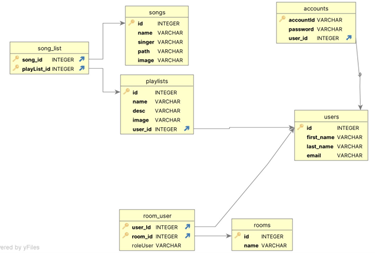
\includegraphics{template_SGU/Picture1.png}}
    %\put(0,-8){\epsfig{width=10mm,figure=hcmut.eps}}
   \end{picture}&
\begin{itemize}
    \item Bảng accounts: lưu trữ thông tin tài khoản của người dùng
\end{itemize}
\begin{tabular}{cllll}
\toprule
  STT & Tên thuộc tính  & Loại & Kiểu & Diễn giải   \\
  \midrule
    1    & accountId  & Khóa chính & varchar & Mã tài khoản \\
  2  & password   &  & varchar & Mật khẩu \\
 3   & user\_id & Khóa ngoại & integer & Mã người dùng\\
   \bottomrule
\end{tabular}

\begin{itemize}
    \item Bảng users: lưu trữ thông tin của người dùng
\end{itemize}
\begin{tabular}{cllll}
\toprule
  STT & Tên thuộc tính  & Loại & Kiểu & Diễn giải   \\
  \midrule
    1    & id  & Khóa chính & integer & Mã người dùng \\
  2  & first\_name   &  & varchar & Tên người dùng \\
 3   & last\_name &  & varchar & Họ người dùng\\
 4 & email &  & varchar & Email người dùng \\
   \bottomrule
\end{tabular}

\begin{itemize}
    \item Bảng rooms: lưu trữ thông tin của phòng nhạc do người dùng tạo
\end{itemize}
\begin{tabular}{cllll}
\toprule
  STT & Tên thuộc tính  & Loại & Kiểu & Diễn giải   \\
  \midrule
    1    & id  & Khóa chính & integer & Mã phòng \\
  2  & name   &  & varchar & Tên phòng \\
   \bottomrule
\end{tabular}

\begin{itemize}
    \item Bảng room\_user: cho biết người dùng thuộc phòng nào và vai trò của người dùng trong phòng nhạc
\end{itemize}
\begin{tabular}{cllll}
\toprule
  STT & Tên thuộc tính  & Loại & Kiểu & Diễn giải   \\
  \midrule
    1    & user\_id  & Khóa chính, khóa ngoại & integer & Mã người dùng \\
  2  & room\_id   & Khóa chính, khóa ngoại & integer & Mã phòng \\
 3   & roleUser &  & varchar & Vai trò của người dùng\\
   \bottomrule
\end{tabular}

\begin{itemize}
    \item Bảng songs: lưu trữ các bài nhạc của phần mềm
\end{itemize}
\begin{tabular}{cllll}
\toprule
  STT & Tên thuộc tính  & Loại & Kiểu & Diễn giải   \\
  \midrule
    1    & id  & Khóa chính & integer & Mã bài hát \\
  2  & name   &  & varchar & Tên bài hát \\
 3   & singer &  & varchar & Tên ca sĩ\\
 4 & path &  & varchar & Đường dẫn \\
  5 & image &  & varchar & Hình ảnh \\
   \bottomrule
\end{tabular}

\begin{itemize}
    \item Bảng playlists: lưu trữ danh sách nhạc do người dùng tạo
\end{itemize}
\begin{tabular}{cllll}
\toprule
  STT & Tên thuộc tính  & Loại & Kiểu & Diễn giải   \\
  \midrule
    1    & id  & Khóa chính & integer & Mã danh sách \\
  2  & name    &  & varchar & Tên danh sách  \\
 3   & desc &  & varchar & Mô tả\\
 4 & image &  & varchar & Đường dẫn hình ảnh \\
  5 & user\_id & Khóa ngoại & integer & Mã người dùng \\
   \bottomrule
\end{tabular}

\begin{itemize}
    \item Bảng song\_list: cho biết danh sách nhạc của người dùng và danh sách các bài hát do người dùng thêm vào
\end{itemize}
\begin{tabular}{cllll}
\toprule
  STT & Tên thuộc tính  & Loại & Kiểu & Diễn giải   \\
  \midrule
    1    & song\_id  & Khóa chính, khóa ngoại & integer & Mã bài hát \\
  2  & playlist\_id    & Khóa chính, khóa ngoại & integer & Mã danh sách  \\
   \bottomrule
\end{tabular}

\subsection{Cấu trúc mã nguồn}
Cấu trúc mã nguồn của dự án được thiết kế theo mô hình client-server:
\subsubsection{Phía Server:}
    \begin{picture}
    \put{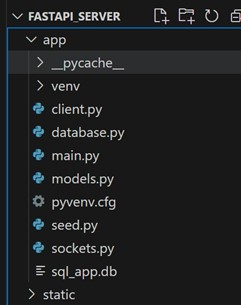
\includegraphics{template_SGU/Picture2.jpg}}
    %\put(0,-8){\epsfig{width=10mm,figure=hcmut.eps}}
   \end{picture}&
\begin{itemize}
    \item    \textbf{\_\_pycache\_\_:}
    Thư mục "pycache" là một thư mục được tạo ra tự động bởi Python 3 để lưu trữ các file bytecode đã được biên dịch (.pyc) khi bạn thực thi một chương trình Python. Bytecode là phiên bản đã được biên dịch của mã nguồn Python và được sử dụng để tăng tốc độ tải và thực thi chương trình.
        \item    \textbf{venv:}
   Công cụ trong Python được sử dụng để tạo môi trường ảo Python. Môi trường ảo là một không gian làm việc cô lập chứa một bản sao của trình biên dịch Python cũng như một bộ thư viện và các công cụ khác cần thiết cho dự án cụ thể. Việc sử dụng môi trường ảo giúp cho việc quản lý các dependencies của dự án trở nên dễ dàng và đảm bảo tính tương thích giữa các phiên bản của các packages khác nhau.
   \item    \textbf{client.py:}
   Kết nối socket đến client
   \item    \textbf{database.py:}
   Kết nối socket đến client 
   \item \textbf{main.py:}
   Đây là hạt nhân của dự án, là nơi khởi động website, cũng là nơi chứa các xử lý chính
   \item \textbf{models.py:}
   File cấu trúc các thực thể từ database
   \item \textbf{seed.py:}
   File tạo dữ liệu cứng cho database
   \item \textbf{socket.py:}
   File thiết lập socket cho dự án
   \item \textbf{sql\_app.db:}
File database được nhúng từ sqlite
   \item \textbf{static:}
   được sử dụng để lưu trữ các tệp tĩnh như CSS, JavaScript, hình ảnh, video và các tài nguyên khác mà không thay đổi trong quá trình chạy ứng dụng.
\end{itemize}

\subsubsection{Phía Client:}
    \begin{picture}
    \put{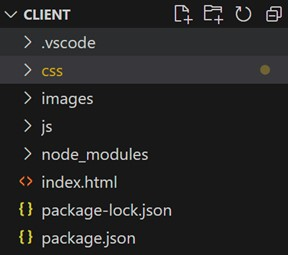
\includegraphics{template_SGU/Picture3.jpg}}
    %\put(0,-8){\epsfig{width=10mm,figure=hcmut.eps}}
   \end{picture}&
\begin{itemize}
    \item    \textbf{css:}
    Nơi lưu trữ các tệp CSS (Cascading Style Sheets) trong một dự án web.
        \item    \textbf{images:}
   Được sử dụng để lưu trữ các tệp hình ảnh trong dự án.
   \item    \textbf{js:}
   Nơi lưu trữ các tệp JavaScript trong một dự án.
   \item    \textbf{node\_modules:}
   Nơi chứa tất cả các modules (các gói) của dự án. 
   \item \textbf{index.html:}
   File "index.html" là trang chính của trang web
   \item \textbf{package-lock.json:}
  Tệp JSON mà npm tự động tạo ra để đảm bảo rằng một bản cụ thể của dependencies sẽ được cài đặt trong môi trường phát triển và triển khai.
   \item \textbf{package.json:}
   Tệp JSON chứa thông tin về dự án, bao gồm các dependencies, scripts, thông tin tác giả, phiên bản, và nhiều thông tin khác.
\end{itemize}

\subsection{Mô hình ứng dụng }
\textbf{Mô hình Client - Server là gì?}
Là mô hình mạng máy tính trong đó các máy tính con được đóng vai trò như một máy khách, chúng làm nhiệm vụ gửi yêu cầu đến các máy chủ. Để máy chủ xử lý yêu cầu và trả kết quả về cho máy khách đó.

\subsubsection{Nguyên lý hoạt động của mô hình:}
Khách hàng (Client) hoạt động như sau:
\begin{itemize}
    \item Người dùng mở ứng dụng trên thiết bị của mình.
    \item Tương tác với giao diện người dùng để gửi yêu cầu như nghe nhạc, tải lên video, hoặc gửi yêu cầu detect.
    \item Gửi yêu cầu đến máy chủ thông qua giao thức truyền thông như HTTP hoặc WebSocket.
    \item Đợi nhận phản hồi từ máy chủ và hiển thị dữ liệu hoặc thông báo tương ứng.

\end{itemize}
Máy chủ (Server) hoạt động như sau:
\begin{itemize}
    \item Tiếp nhận yêu cầu từ khách hàng thông qua các cổng kết nối được xác định.
    \item Xử lý yêu cầu dựa trên logic nghiệp vụ của ứng dụng.
    \item Truy xuất hoặc cập nhật dữ liệu trong cơ sở dữ liệu nếu cần.
    \item Phản hồi lại cho khách hàng bằng cách cung cấp dữ liệu hoặc thực hiện các hành động tương ứng.
\end{itemize}

\subsubsection{Ưu điểm}
\begin{itemize}
    \item Giúp chúng ta có thể làm việc trên bất kì một máy tính nào có hỗ trợ giao thức truyền thông. Giao thức chuẩn này cũng giúp các nhà sản xuất tích hợp lên nhiều sản phẩm khác nhau mà không gặp phải khó khăn gì.
    \item Có thể có nhiều server cùng làm một dịch vụ, chúng có thể nằm trên nhiều máy tính hoặc một máy tính.
    \item Chỉ mang đặc điểm của phần mềm mà không hề liên quan đến phần cứng, ngoài yêu cầu duy nhất là server phải có cấu hình cao hơn các client.
    \item Hỗ trợ người dùng nhiều dịch vụ đa dạng và sự tiện dụng bởi khả năng truy cập từ xa.
    \item Cung cấp một nền tảng lý tưởng, cho phép cung cấp tích hợp các kỹ thuật hiện đại như mô hình thiết kế hướng đối tượng, hệ chuyên gia, hệ thông tin địa lý (GIS).
\end{itemize}

\subsubsection{Kết luận:}
Mô hình client-server là một mô hình phổ biến và mạnh mẽ trong phát triển ứng dụng, đặc biệt là đối với ứng dụng như hệ thống nghe nhạc và detect video. Sự phân tán, tính linh hoạt và khả năng mở rộng của mô hình này là những ưu điểm quan trọng, mặc dù cũng cần cân nhắc về độ trễ và sự phụ thuộc vào máy chủ. Vì vậy mô hình này rất phù hợp cho việc xây dựng ứng dụng này 

\subsection{Các tính năng được xây dựng}
- Nghe Nhạc Cá Nhân:
\begin{itemize}
    \item Cho phép người dùng tạo danh sách phát, lưu trữ và phát nhạc cá nhân.
    \item Thực hiện các chức năng như play, pause, skip.
    \item Tham gia vào các phòng nhạc để thưởng thức âm  nhạc cùng nhau
\end{itemize}
- Detect Video:
\begin{itemize}
    \item Cho phép người dùng đẩy video lên hệ thống để tiến hành nhận diện nội dung video.
    \item Hỗ trợ nhận dạng các đối tượng, khuôn mặt, hoặc hành động trong video.
\end{itemize}
- Tải video về:
\begin{itemize}
    \item Sau khi quá trình detect video hoàn tất, người dùng có thể tải về kết quả đã detect về lại máy.
\end{itemize}
- Phòng Nghe Nhạc:
\begin{itemize}
    \item Tạo ra các phòng nghe nhạc cho người dùng có thể tham gia và chia sẻ âm nhạc cùng nhau.
    \item Phân quyền cho các user trong từng phòng nhạc
\end{itemize}
- Quản Lý Tài Khoản:
\begin{itemize}
    \item Cho phép người dùng đăng ký, đăng nhập
\end{itemize}


\section{HIỆN THỰC}
\subsection{Cài đặt thư viện}
Trong quá trình phát triển dự án, chúng em đã sử dụng một số thư viện quan trọng để hỗ trợ việc xây dựng và triển khai ứng dụng. Dưới đây là danh sách các thư viện cũng như quá trình cài đặt chúng:
\subsubsection{FastAPI:}
\begin{itemize}
    \item FastAPI là một framework nhanh chóng để xây dựng API web với Python 3.6+.
    \item Cài đặt: pip install fastapi
\end{itemize}
\subsubsection{Socket.io:}
\begin{itemize}
    \item Socket.io là một thư viện cho phép giao tiếp thời gian thực giữa client và server.
    \item Cài đặt: npm install socket.io
\end{itemize}
\subsubsection{SQLAIchemy:}
\begin{itemize}
    \item SQLAlchemy là một thư viện ORM mạnh mẽ cho Python, giúp làm việc với cơ sở dữ liệu dễ dàng hơn.
    \item Cài đặt: pip install sqlalchemy
\end{itemize}
\subsubsection{Ultralytics:}
\begin{itemize}
    \item Ultralytics là một bộ công cụ hỗ trợ trong việc phát triển các mô hình Deep Learning.
    \item Cài đặt: pip install ultralytics
\end{itemize}
\subsubsection{Pillow (PIL):}
\begin{itemize}
    \item Pillow là một thư viện Python cho xử lý hình ảnh.
    \item Cài đặt: pip install pillow
\end{itemize}
Với việc cài đặt các thư viện trên, chúng em đã có các công cụ cần thiết để triển khai các chức năng trong ứng dụng của mình một cách hiệu quả và linh hoạt.

\subsection{Các tính năng chính của ứng dụng}
\begin{itemize}
    \item Tạo playlist\\
        \begin{picture}
    \put{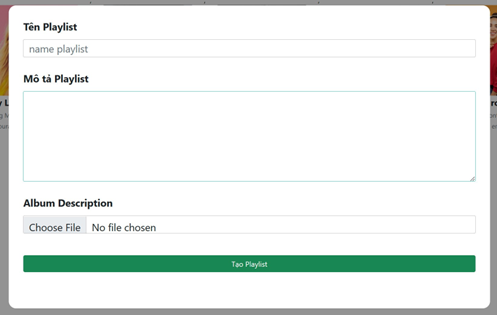
\includegraphics{template_SGU/Picture4.png}}
    %\put(0,-8){\epsfig{width=10mm,figure=hcmut.eps}}
   \end{picture}&
   \item Tất cả playlist\\
       \begin{picture}
    \put{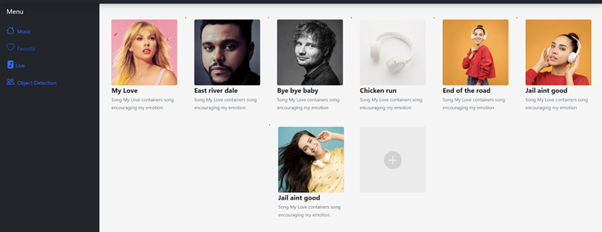
\includegraphics{template_SGU/Picture5.png}}
    %\put(0,-8){\epsfig{width=10mm,figure=hcmut.eps}}
        \put{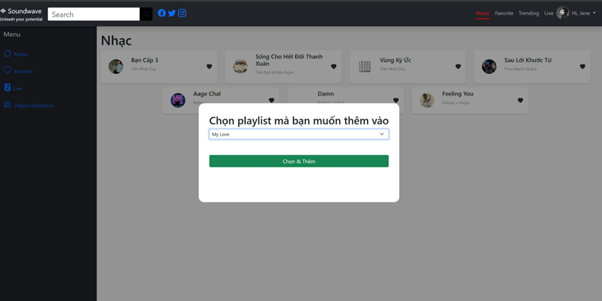
\includegraphics{template_SGU/Picture6.png}}
    %\put(0,-8){\epsfig{width=10mm,figure=hcmut.eps}}
   \end{picture}&
   \item Phòng nghe nhạc \\
           \begin{picture}
    \put{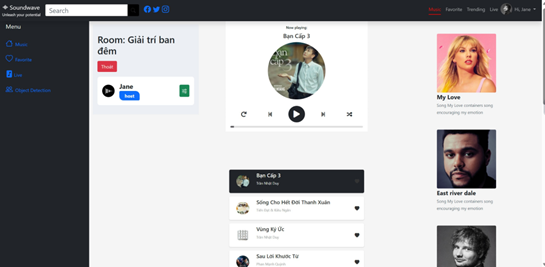
\includegraphics{template_SGU/Picture7.png}}
    %\put(0,-8){\epsfig{width=10mm,figure=hcmut.eps}}
   \end{picture}&
   \item Sảnh chờ vào phòng nghe nhạc của các thành viên\\
           \begin{picture}
    \put{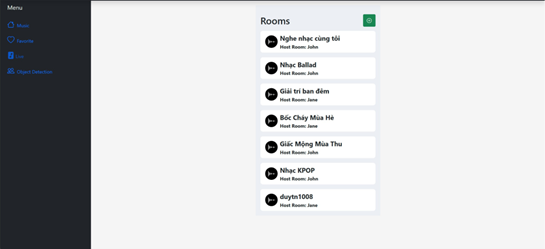
\includegraphics{template_SGU/Picture8.png}}
    %\put(0,-8){\epsfig{width=10mm,figure=hcmut.eps}}
   \end{picture}&
   \item Upload video để detect\\
           \begin{picture}
    \put{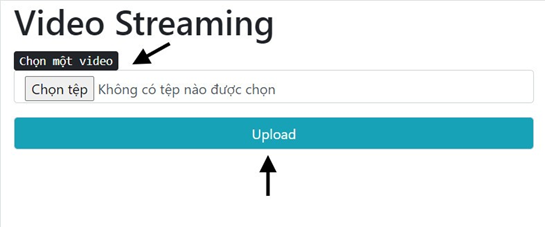
\includegraphics{template_SGU/Picture9.png}}
    %\put(0,-8){\epsfig{width=10mm,figure=hcmut.eps}}
   \end{picture}&
   \item Chờ hệ thống xử lý: \\
           \begin{picture}
    \put{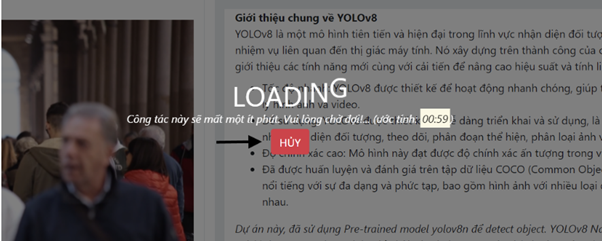
\includegraphics{template_SGU/Picture10.png}}
    %\put(0,-8){\epsfig{width=10mm,figure=hcmut.eps}}
   \end{picture}&
   \item Download video sau khi detect:\\
           \begin{picture}
    \put{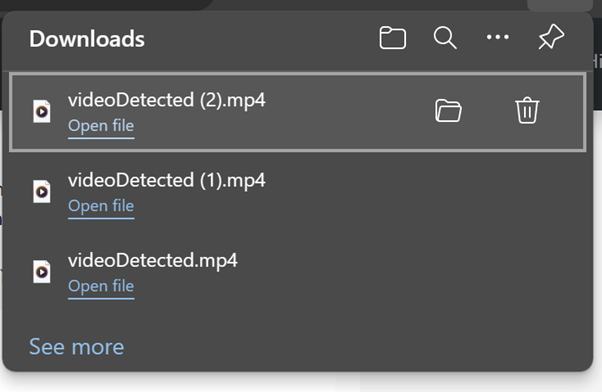
\includegraphics{template_SGU/Picture11.png}}
    %\put(0,-8){\epsfig{width=10mm,figure=hcmut.eps}}
   \end{picture}&
   \item Chọn vật thể để detect: \\
           \begin{picture}
    \put{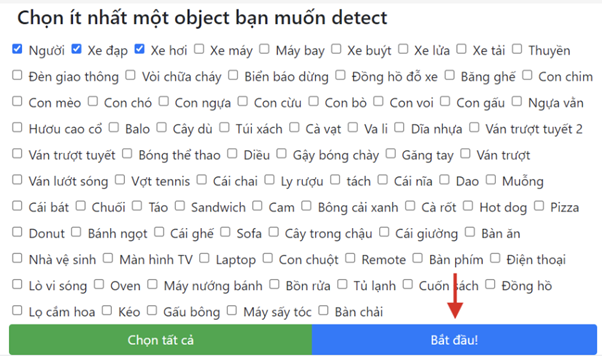
\includegraphics{template_SGU/Picture12.png}}
    %\put(0,-8){\epsfig{width=10mm,figure=hcmut.eps}}
   \end{picture}&
    \item Video sau khi detect:\\
            \begin{picture}
    \put{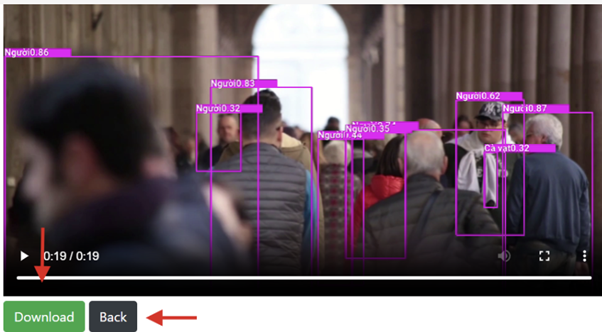
\includegraphics{template_SGU/Picture13.png}}
    %\put(0,-8){\epsfig{width=10mm,figure=hcmut.eps}}
   \end{picture}&
   \item Phân quyền: \\
           \begin{picture}
    \put{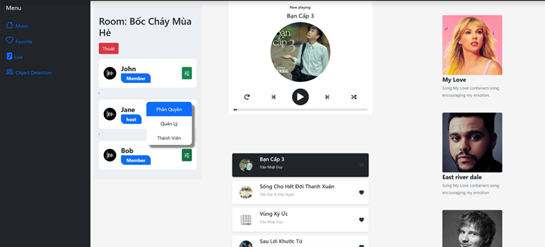
\includegraphics{template_SGU/Picture14.png}}
    %\put(0,-8){\epsfig{width=10mm,figure=hcmut.eps}}
   \end{picture}&
   \Item Cửa sổ đăng nhập, đăng ký: \\
           \begin{picture}
    \put{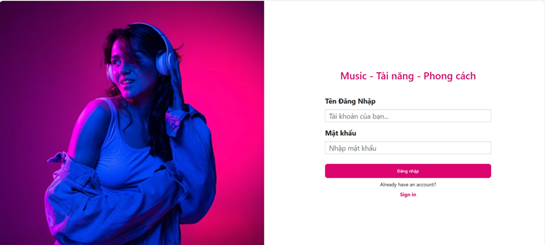
\includegraphics{template_SGU/Picture15.png}}
    %\put(0,-8){\epsfig{width=10mm,figure=hcmut.eps}}
   \end{picture}&
\end{itemize}


\section{KẾT LUẬN}
\subsection{Kết quả đạt được và mức độ đáp ứng mục tiêu của dự án}
Dự án của chúng em đã đạt được những chức năng cơ bản. Trang web đã cung cấp được những nhu cầu giải trí và làm việc cơ bản cho người dùng như:
\begin{itemize}
    \item Nhận diện các đối tượng trong viddeo thông qua hình thức streaming và phân tích được độ chính xác (\%) của vật thể theo các lựa chọn đối tượng có sẵn
    \item Sau khi hệ thống xử lý video, người dùng có thể download video đã được xử lý
    \item Có các chức năng tạo và xóa playlist. Thêm và xóa các bài nhạc vào playlist theo mong muốn, sở thích
    \item Tìm kiếm các bài nhạc dễ dàng để thêm vào playlist
    \item Tạo phòng nghe nhạc (ứng dụng socket), người dùng có thể tham gia vào phòng dựa vào các chủ đề yêu thích của bản thân. Người dùng cũng có thể phát các bài nhạc theo playlist của riêng bản thân cho các thành viên trong phòng cùng thưởng thức (nếu được sự ủy quyền của chủ phòng)
    \item Người dùng là chủ phòng có thể xóa các thành viên trong phòng, phân quyền cho các thành viên trong phòng
\end{itemize}
\subsection{Bảng phân công công việc}
\begin{tabular}{llll}
\toprule
  Họ và tên & MSSV  & Công việc & Tỉ lệ đóng góp\\
  \midrule
   Nguyễn Vũ Tiến Đạt    & 3121410148  & Module nhạc & 25\% \\
 Trần Nhật Duy  &3121410125   & Module socket phòng nghe nhạc & 25\% \\
 Nguyễn Hoàng Tiến   & 3121560090 & Detect Object &  25\%\\
 Nguyễn Hoàng Kiều Ngân & 3121560056 & Module playlist & 25\% \\
   \bottomrule
\end{tabular}
\end{document}

